\documentclass{article}

\usepackage{amsmath}
\usepackage{amsthm}
\usepackage{hyperref}
\usepackage{graphicx}

\usepackage{amssymb}

\newcommand{\dxdy}[2]{\frac{d #1}{d #2}}
\newcommand{\pdxdy}[2]{\frac{\partial #1}{\partial #2}}
\newcommand{\liminfty}[1]{\lim_{#1 \to \infty}}

\newcommand{\abs}[1]{\left \vert #1 \right \vert}
\newcommand{\norm}[1]{\left \Vert #1 \right \Vert}
\DeclareMathOperator{\sign}{sign}

\newtheorem{thm}{Theorem}

\begin{document}

\section{Fixed point iterations}

We examine in detail two fixed point iterations:
\begin{equation} \label{eq:FPI}
g_1(z) = e^{-z}, \quad g_2(z) = -\log(z).
\end{equation}
First and foremost, these functions have fixed points at the real root of
\begin{equation} \label{eq:f}
z e^z - 1 = 0
\end{equation}
and are inverses of each other.

The function $g_1(z)$ is $2 \pi$--periodic in the imaginary direction.
It is for this reason that it cannot converge to any of the complex roots of function \ref{eq:f}.
Likewise, this means we need only consider $-\pi \leq Im(z) < \pi$.
The function $g_2(z)$ also does not converge to complex roots by choice of branch cut.
This can be changed with the addition of $i n 2 \pi$, where $n$ is the branch cut of interest.

We are concerned with where each function will converge.
We can guarantee convergence in a region $D$ by the fixed point theorem.

\begin{thm}[Fixed point iteration theorem] \label{thm:fpi}
If a function $g(z)$ satisfies
\begin{description}
\item[(i)] $g(z) \in D$
\item[(ii)] $\abs{g'(z)} < 1$
\end{description}
for all $z \in D$ then it has a unique fixed point in $D$ and the iteration $z_{n+1} = g(z_n)$ converges to this fixed point.
\end{thm}

Consider $g_1(z)$:
condition (ii) of theorem \ref{thm:fpi} is satisfied when $Re(z) > 0$;
for condition (i) note that $g_1(z)$ rotates off the real axis by angle $-Im(z)$.
For $g_1(z)$ to satisfy $Re(g_1(z)) > 0$ it is necessary that $\abs{Im(z)} < \pi/2$.
Our region $D_0$ (the region for which $g_1(z)$ satisfies theorem \ref{thm:fpi}) is therefore:
\begin{equation} \label{eq:D1}
D_0 = \{ z \in \mathbb{C} \vert Re(z) > 0, \ -\pi/2 < Im(z) < \pi/2 \} .
\end{equation}
Given that $g_2(z)$ is the inverse of $g_1(z)$ and $D_0$ exists, there is no such region for $g_2(z)$.

\begin{figure}
	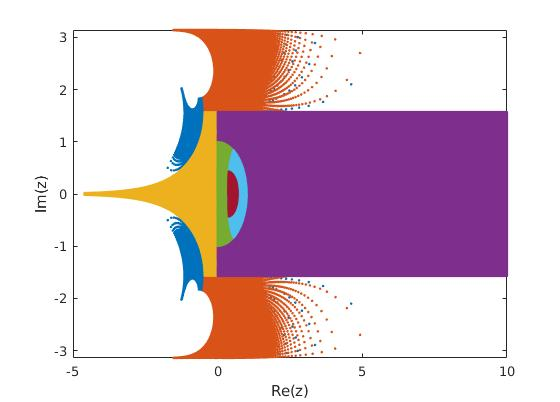
\includegraphics[width=\textwidth]{FPI_01.jpg}
	\caption{The region $D_0$ and its images under $g_1(z)$ and $g_2(z)$.}
	\label{fig:fpi01}
\end{figure}

Figure \ref{fig:fpi01} gives a representation of the region $D_0$ (purple) and its images and pre-images.
For ease of notation we define the sets $D_k$ as:
\begin{equation*}
D_{k+1} = g_1(D_k), \quad D_{k-1} = g_2(D_k).
\end{equation*}
Since $D_1 \subset D_0$ by definition of $D_0$ and $g_2(g_1(z)) = z$ there exists a hierarchy of sets:
$D_{k+1} \subset D_k \subset D_{k-1}$ for all $k \in \mathbb{Z}$.
Each set $D_{k-1}$ is the pre-image of $D_k$ under the $g_1(z)$ function.
As such, $D_{-\infty}$ represents the basin of attraction of $g_1(z)$.

\section{Preconditioned Newton}

We now look at applying Newton's method to the functions $g_1(z) - z$ and $g_2(z) - z$.
This will give the following fixed point iteration functions:
\begin{equation} \label{eq:Newton}
f_1(z) = \frac{z g_1'(z) - g_1(z)}{g_1'(z) - 1} = \frac{1 + z}{1 + e^z}, \quad f_2(z) = \frac{z ( 1 - \log(z) )}{1 + z} .
\end{equation}
Note that $f_1(z) = f_2(e^{-z})$ and $f_2(z) = f_1(-\log(z))$.

The function $f_1(z)$ has singularities at all branches of $\log(-1)$.
Unlike $g_1(z)$, it is not periodic in the imaginary direction.
The function $f_2(z)$ has an erroneous fixed point at $z=0$, a singularity at $z=-1$ and a root at $z = e$.
These points will be problematic and must be excluded from the basins of attraction.

We can perform the same analysis as before using theorem \ref{thm:fpi}.
Condition (ii) can be written in terms of the fixed point functions:
\begin{equation*}
\abs{f_1'(z)} = \abs{ \frac{ g_1''(z) (g_1(z) - z) }{ (g_1'(z) - 1)^2 } } < 1, \quad \abs{ \frac{ g_2''(z) (g_2(z) - z) }{ (g_2'(z) - 1)^2 } } < 1 .
\end{equation*}
This ultimately requires
\begin{equation*}
\abs{f_1'(z)} = \abs{ \frac{1 - z e^z}{(1 + e^z)^2} } < 1, \quad \abs{f_2'(z)} = \abs{ \frac{z + \log(z)}{(1 + z)^2} } < 1.
\end{equation*}

Condition (ii) holds for $f_2(z)$ except in an elliptical region containing $z=-1$.
The region where the fixed point theorem is true for $f_2(z)$, hereafter called $D_0^2$, is then the complex plane without the pre-images of this ellipse.
However, if $z \approx -1$ but not equal then $f_2(z)$ is not within this ellipse.
More precisely, the image of the ellipse is outside the ellipse.
Thus, $D_0^2$ is the entire complex plane except for the points -1, 0 and $e$ and their pre-images.
This constitutes a countable set.
(side note: the pre-image of 0 for $f_2(z)$ is $e$, so the definition of $D_0^2$ can be further simplified if desired)

Analysis for $f_1(z)$ is carried out numerically.
Through experiments we can establish that the ball of radius 1 in the complex plane represents a region where theorem \ref{thm:fpi} is satisfied.
Call this ball $D_0^1$.
We can also show that the inverse of $f_1(z)$ is
\begin{equation*}
f_1^{-1}(z) = z - 1 - W(-z e^{z-1})
\end{equation*}
where $W(z)$ is the Lambert W function (0 branch).
Using this, we repeat figure \ref{fig:fpi01}.

\begin{figure}
	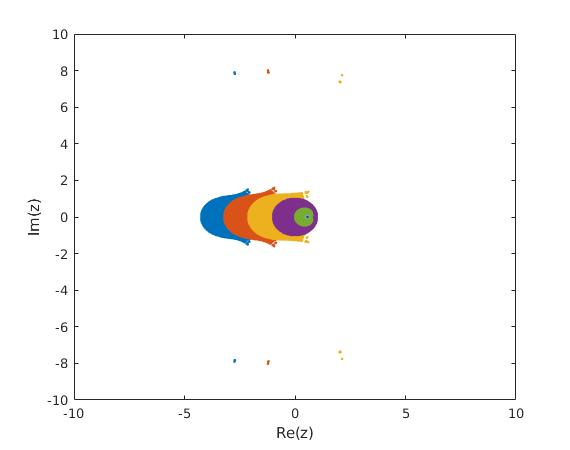
\includegraphics[width=\textwidth]{FPI_02.jpg}
	\caption{The region $D_0^1$, its images and pre-images under $f_1(z)$.}
	\label{fig:fpi02}
\end{figure}

Figure \ref{fig:fpi02} shows the hierarchy of sets, with $D_0^1$ in purple.
Its images are inset and converge rapidly to the root.
Its pre-images extend onto the negative real line with some scattering.
A more resolved $D_0^1$ (see figure \ref{fig:fpi03}) shows greater detail in this scattering, and reveals some fractal structure.

\begin{figure}
	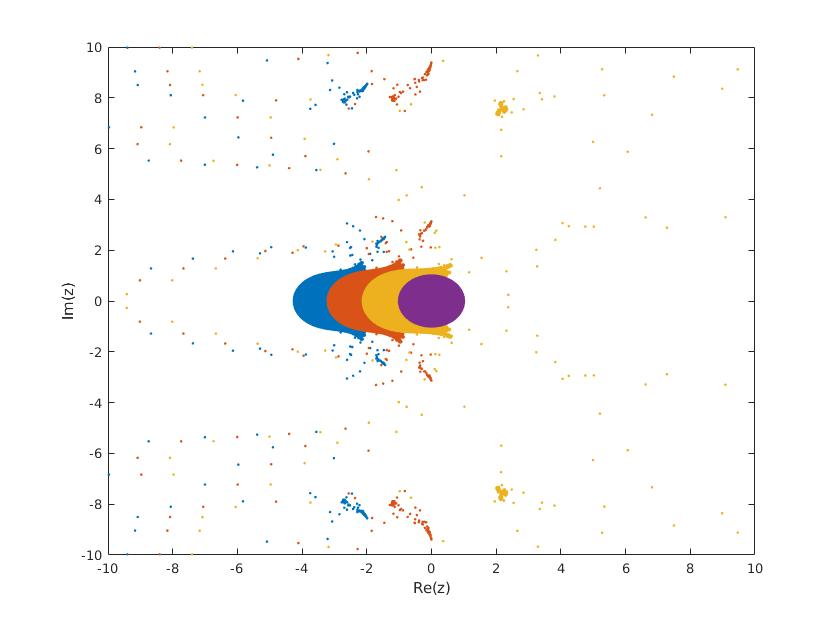
\includegraphics[width=\textwidth]{FPI_03.jpg}
	\caption{The region $D_0^1$ and its pre-images under $f_1(z)$.}
	\label{fig:fpi03}
\end{figure}

\end{document}